%% Quick build: [path]/convert.sh|pdflatex -synctex=1 -interaction=nonstopmode %.tex|biber %.bcf|pdflatex -synctex=1 -interaction=nonstopmode %.tex|pdflatex -synctex=1 -interaction=nonstopmode %.tex|evince %.pdf

\documentclass[doc]{apa6}
\usepackage[utf8]{inputenc}
\usepackage[english]{babel}
\usepackage{csquotes}
\usepackage[style=apa,sortcites=true,sorting=nyt,backend=biber]{biblatex}

\usepackage{amsmath}
\usepackage{amsfonts}
\usepackage{amssymb}
\usepackage{gensymb}
\usepackage[load=abbr]{siunitx}
\usepackage{setspace}	% for line spacing
\usepackage{calc}		% for figure scaling
\usepackage{svg}		% for graphics
\usepackage{graphicx}	% for graphics
\usepackage[left=1in,right=1in,top=1in,bottom=1in]{geometry}
\usepackage{listings}

\DeclareLanguageMapping{american}{american-apa}
\addbibresource{/home/rob/Documents/bibtex/library.bib}

\linespread{1.5}

% Images are build by calling images/generate.sh <images> <output> where
% output is the "build" directory used by Texmaker.
\graphicspath{{./build/images/}}

\DeclareUnicodeCharacter{2010}{ }

%\lstset{%
%  basicstyle=\small\ttfamily,
%  language=Python
%}



\shorttitle{}

\title{Utilizing Cubic Splines for Vertical Control of Remote-Sensing Unmanned Aerial Vehicles}
\author{Rob Skelly}
\affiliation{University of Victoria}

\keywords{Cubic Splines,UAV,Remote Sensing}

\abstract{
	etc...
}

\begin{document}

\maketitle

\section{Problem Statement}

In the field of remote sensing with unmanned aerial vehicles (UAVs), the maintenance of data quality is of primary importance and can be managed, in part, by stabilising the instrument-to-subject distance and orientation. This can be accomplished by controlling the vehicle's altitude and attitude, respectively.

Flight plans for UAV surveys are generally pre-planned using purpose-built software and followed (semi-) automonmously by the aircraft. Most currently-available software allows the creation of flight plans only in the horizontal plane \parencite[e.g.,][]{ArduPilot2018,DJI2018a,Microdrones2018,Group2018,UAVToolbox2018}, leaving it to the pilot to set a constant -- usually barometric -- altitude sufficient to clear the terrain and any obstacles in the study area. Those packages that do enable terrain avoidance rely on an  existing digital elevation model (DEM) \parencite[e.g.,][]{PrecisionHawk2018,UgCS2018,MapsMadeEasy2018}, or use a nadir-aligned rangefinder for \emph{reactive} terrain avoidance.

In the remote sensing context, \emph{terrain avoidance} is distinct from, and inferior to, \emph{surface following}: the objective is not merely to avoid colliding with the terrain, but to maintain an altitude and attitude with respect to the sensed surface (which may be a vegetative canopy or the terrain itself) which preserves the quality -- image scale and distortion, point density, signal-to-noise ratio, swath overlap, etc. -- of the data products. Given limitations on the energy-density of current batteries, and thus flight duration, the ability to follow a trajectory safely and efficiently is also a major concern.

This research pursues the development of a real-time, predictive flight-planning system for UAV remote sensing, to satisfy the data-quality objectives of a remote-sensing mission while resolving some of the inadequacies of existing mission-planning software packages. The system will use a forward-looking laser rangefinder to generate a two-dimensional point cloud from which a trajectory will be computed, in the form of a piecwise cubic spline. 

Specifically, this proposal outlines a rationale and methodology for selecting the type of spline (e.g., interpolating, smoothing, natural, constrained, weighted) whose characteristics best satisfy the data-quality, efficiency and safety constraints as described. 

\section{Background}

\subsection{UAV Remote Sensing}

Unmanned aerial vehicles (UAVs) are small reusable aircraft, controlled remotely by a human operator or (semi-)autonomously, which can range in size from insect-scale to jet-powered military aircraft \parencite{Avadhanula2002,Deng2003} and are subject to an ongoing explosion in engineering, scientific, military and commercial interest. 

Military interest in UAV research is a given and indeed drives much of the development of related technologies. Perhaps surprisingly, the development in UAVs began in 1916 and continued with the support of the United States military, culminating in extensive utilization of UAVs during the war in Vietnam \parencite{Valavanis2007,Cook2007} and continuing into the 21st century in the Middle East. 

More recently, the emergence of an entrepreneurial, just-build-it technological culture and the ability of firms to design and produce highly sophisticated, miniaturized components and high-capacity, lightweight batteries, has enabled basement tinkerers, commercial startups and academics alike exploit the capabilities offered by UAVs, rapidly and at little cost.

%In particular, the availability of compact, low-power computers with high processing speeds, along with advances in real-time operating systems, have enabled the development of flight-control systems which can safely %manage the inherent instability of multi-rotor aircraft. The proliferation of ``system on a chip'' (SoC) options, including environmental sensors, accelerometers, gyroscopes and magnetometers facilitiates the %production of compact sensing instruments and inertial measurement units suitable for flight control. Compact, reliable laser rangefinders and spectrometers are becoming available and accessible at affordable prices. %Finally, advances in battery technology are finally providing energy density and light weight that could previously be attained only with hydrocarbon fuels (and the deleterious vibration caused by reciprocating %engines.) Importantly, one does not need access to electrical engineering knowledge, nor to private production facilities, to produce the sophisticated electronic hardware required for building a remote-sensing UAV. %The building blocks are small enough, cheap enough and accurate enough that almost anyone can build a sensor package to their requirements.

In the scientific remote-sensing field, where the execution of an aerial survey could entail hundreds of thousands of dollars in costs for planning, permitting, instrumentation, pilots and aircraft, the advent of UAVs provides researchers with the opportunity to conduct research at much lower cost with little turnaround time. Naturally, there are compromises to be made between traditional aerial remote-sensing and the use of UAVs. The latter tend to be limited to low altitudes, short flight durations and small site sizes. The instrumentation -- specifically multi- and hyperspectral imagers and LiDAR -- has only recently achieved a level of quality sufficient for research, and form factor small and light enough for inclusion on a UAV. Additionally, many of these instruments are designed for uses other than remote sensing, in particular LiDAR devices, which are often designed for the automotive market. However, with the drawbacks come advantages. The level of detail attainable with a low-altitude UAV survey would be impossible given the cost, danger and disruption of a low-altitude survey using conventional aircraft.

Traditional aerial surveys have the advantage that, at typical survey altitudes of $\SI{250}\m-\SI{1000}\m$, variations in terrain relief and vegetation canopy height (collectively, surface height) are insignificant relative to the platform altitude -- except in extreme cases, such as alpine terrain -- causing minimal scale distortion in the resulting imagery. Low-altitude UAV surveys, which may take place at $\SI{10}\m-\SI{50}\m$ above the surface, encounter much larger relative variations in surface height and so must follow the surface, both to maintain data quality and to avoid colliding with it. In addition, because there are many structures, both natural and human-made, that may project above a UAV's trajectory, the vehicle must have the ability to detect and avoid hazards. Manned aircraft, with an alert pilot and high altitude, rarely face such obstacles. 

\subsection{Data Quality}

The quality of remotely-sensed data can be quantified in a number of ways. The average posting distance, or point density, of a LiDAR point cloud contributes to the power of any statistical derivatives; spectral imagery can be affected by variations in atmospheric attenuation, scale distortions and signal-to-noise fluctuations; and the degree of overlap between swaths can vary. These are attributable to variations in the platform velocity, altitude and attitude which, as the instruments are fixed to the airframe, which must be carefully maintained by the flight controller. In general, the lower the nominal altitude, for a given site, the larger the effect of surface height variation on data quality.

A final important aspect of data quality is time-of-collection. A spectral survey is ideally conducted as near as possible to solar noon under stable atmospheric conditions. A researcher must be opportunistic and maximise productivity during ideal conditions. Repeating a survey to produce a DEM or terrain following, or interrupting one to change batteries, may delay the completion of the survey or limit the size of the study site, and splitting the survey over multiple days risks a change in the weather. Maximising the power efficiency of a survey, while minimizing its duration, are imperative, as is eliminating the need to repeat a survey to produce a DEM for terrain avoidance.

\subsection{Surface Following}

The foregoing quality and efficiency concerns can be resolved, at least in part, by a surface-following system that accurately maintains the altitude of the aircraft above the surface while minimising disturbances to its attitude and velocity. 


Reactive, real-time systems using nadir-aligned rangefinders, cannot anticipate variations surface height and so have no way of forecasting a trajectory that protects data quality while repsecting the physical limitations of the aircraft.

Mission planning packages that allow the selection or production of a digital elevation model (DEM) \parencite[e.g.,][]{PrecisionHawk2018,UgCS2018,MapsMadeEasy2018}, are either tied to coarse, publicly-available datasets, such as the Shuttle Radar Topography Mission (SRTM), or require a pre-flight and subsequent photogrammetric or LiDAR processing to produce a DEM. 

Publicly-available DEMs may be out of date, poorly-documented, incompatible with the working coordinate system and datum or of doubtful provenance. The SRTM mission in particular used C- and X-band radar, which penetrates a vegetative canopy to a variable degree depending on the type of vegetaion, density, gap structure, senescence, wetness and other factors \parencite{Miliaresis2009}, significantly underestimating their height \parencite{Sexton2009}. As well, the SRTM represents the surface of the Earth, at the time of writing, 19 years in the past. 

If a DEM must be produced in the field, a preliminary survey is required, meaning that at least two full surveys must be conducted, plus the processing time required to produce the model. Since the model must be produced first, the researcher has no way of knowing if conditions will still be suitable by the time the second survey is begun. 

A real-time, predictive surface-following system obviates the need for these additional flights, allowing the researcher to conduct surveys during ideal conditions as they arise, and to adapt the flight plan in real-time to accomodate the prevailing conditions.

Any surface-following system must be able to accomodate the different surface charactistics and mission objectives that a researcher may encounter. For example, a vineyard's rows (figure \ref{fig:photo_culmina_rows}) are spaced approximately $\SI{2}\m$ apart, creating a depression between rows. It would be undesireable for the aircraft to descend into the spaces between rows; rather, its trajectory should carry it smoothly over a surface implied by the tops of the rows while it follows the low-frequency variations in the surface (fgure \ref{fig:photo_culmina_rows_slope}). (On the other hand, if the researcher were interested in imaging the sides of each vine as well as the tops, following this high-frequency surface variation would be desirable.) In this sense, a surface-following system is a low-pass filter with configurable sensitivity. 

\begin{figure} %[htbp] % htbp stand for "here", "top", "bottom", "page"
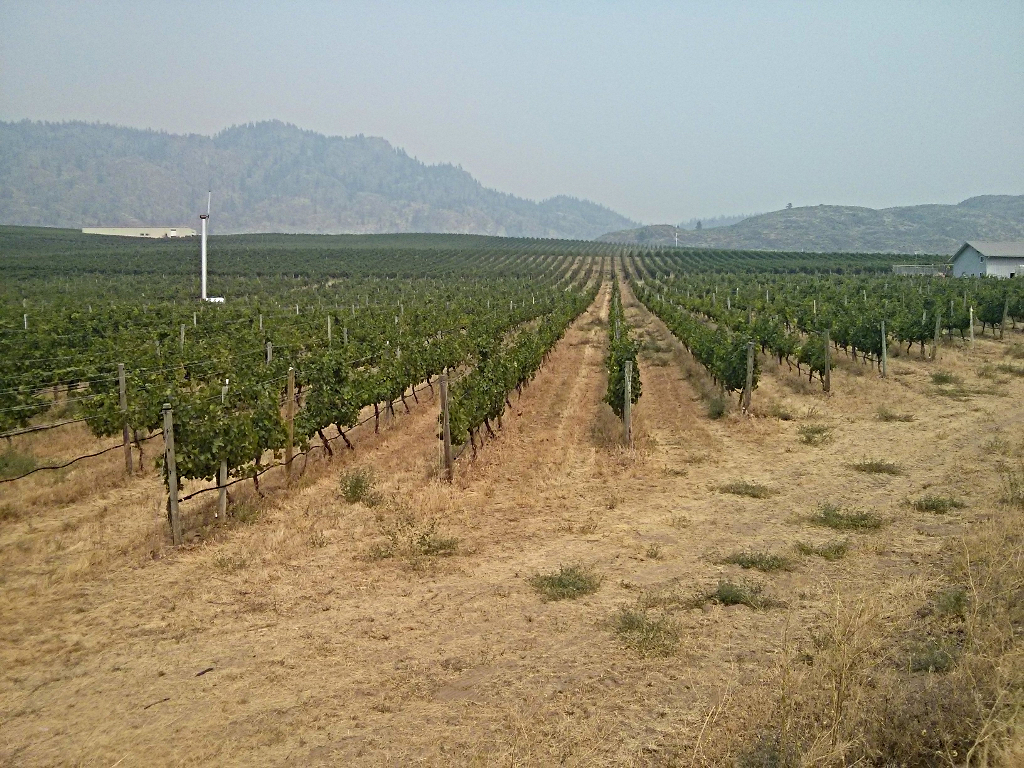
\includegraphics[width=1.0\linewidth]{tmp/photo_culmina_rows.pdf} 
\caption{Typical spacing of vinyard rows. Culmina Winery, Penticton, BC. August 2017.}
\label{fig:photo_culmina_rows}
\end{figure}

\begin{figure} %[htbp] % htbp stand for "here", "top", "bottom", "page"
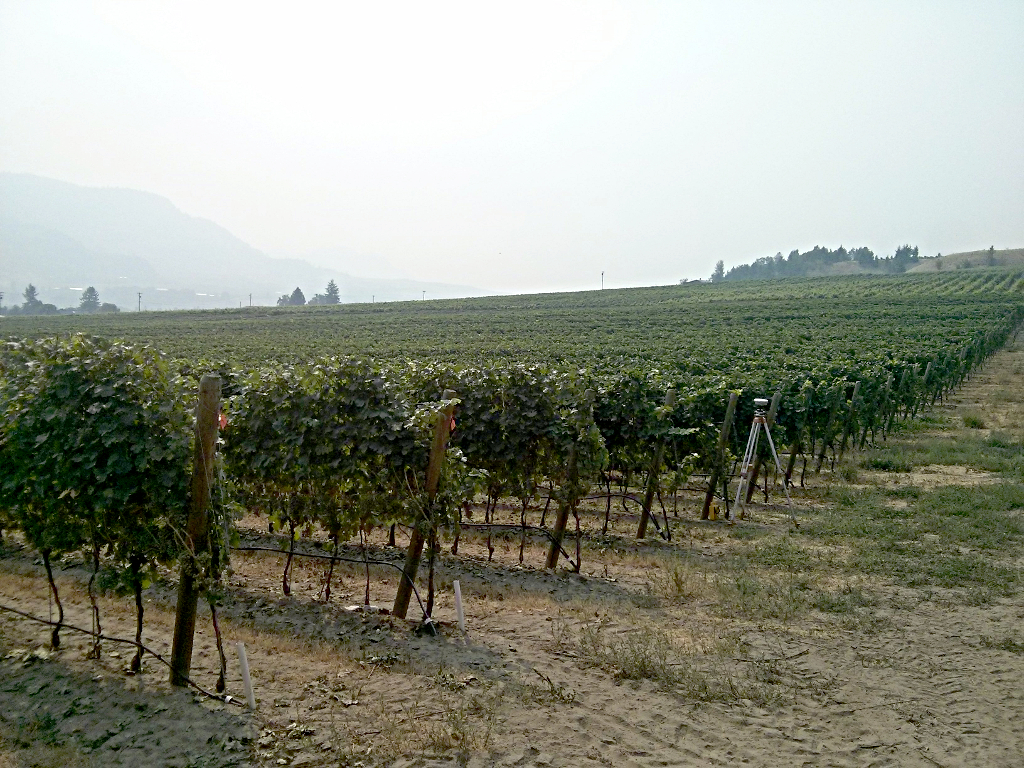
\includegraphics[width=1.0\linewidth]{tmp/photo_culmina_rows_slope.pdf} 
\caption{Low-frequency surface height variation, Culmina Winery, Penticton, BC. August 2017.}
\label{fig:photo_culmina_rows_slope}
\end{figure}

\subsection{Cubic Splines}

The word ``spline'' originates in drafting, where long, flexible wooden beams, called splines, were used to model curves. A spline would be placed on the drawing, held down by two or more lead weights called ``ducks,'' and would seek a shape which minimized the energy stored in the beam. In this sense, the spline could be considered an optimal interpolator \parencite{Wegman2016}. 

In mathematics, the spline is consists of a set of piecewise (usually cubic) polynomials, one each between each pair of ducks, or \emph{knots}. At each intermediate knot, the first, and possibly higher, derivatives of the adjoining polynomials are held equal, resulting an a curve that is smooth and differentiable along its entire length. The minimum-energy constraint is modelled by minimizing mean square curvature of the polynomial \parencite{Wegman2016}.

The mechanical spline and its mathematical equivalent are, of course, interpolators -- they pass through each of the knots. An alternative construction -- the smoothing or approximating spline -- allows the spline to pass through clusters of knots, preserving the overall shape of the data distribution without passing through each knot exactly. 

Weighted cubic spline.

Both the interpolating and smoothing spline are candidates for trajectory construction.

Natural cubic spline S' is 0 at the ends.


\subsection{Surface Reconstruction}

A scanning laser rangefinder is used to generate a point cloud representing the surface to be traversed by the aircraft. The rangefinder is angled forward and down from horizontal (i.e., rotated on the x-axis) to intersect the surface, and will oscillate to the right and left. With accurate angular measurement, this could produce a 3-dimensional point cloud, but this is unnecessary. The points cloud is collapsed in the x-dimension leaving a plane in the y-z. The points along the upper edge of this planar point cloud constitute the ``surface'' for the purpose of navigation.

Where the surface is porous, as in the case of a vegetative canopy, laser returns will indicate not only the ultimate surface, but surfaces beneath it, including intermediate reflectors in the canopy and the terrain itself. This is undesireable, and returns from the ultimate surface must be extracted. 

Once these surface points are isolated, they must be filtered to locate points suitable for use as knots, with the primary consideration being a sufficient inter-knot distance. If the knots are too near to one another in the y-dimension, short splines with radical curvatures or loops may be result, which could be impossible for the aircraft to negotiate.

Two methods of surface-point extraction are proposed: 

\begin{enumerate}
\item Longitudinal binning: a lag distance is selected, which defines a series of ``bins'' of equal width in the y-direction. As each point arrives, it is placed in the appropriate bin. Each bin is represented by the point with the maximum z-coordinate. All others are discarded. The y-coordinate of the point is replaced by the coordinate of the bin's centre.
\item Concave hull: the lag distance is used to limit the length of segments produced by a Graham-scan convex hull operation on the surface. 
\end{enumerate}

The first strategy ensures that the knots are equidistant and that each knot matches the height of highest obstacle in the vicinity. This method is higly efficient, as the binning process is implied by simply truncating the y-coordinate of each point and checking the magnitude of its z-coordinate. However the knots extracted by this method are biased upwards: a maximum can be higher than the true surface if it is displaced from its original y-coordinate but not lower. If the points are not so displaced, there is a risk that two points in adjacent bins can form too steep a slope. This could exclude the interpolating spline as a valid trajectory.


Though the second strategy is more computationally intensive than binning, Andrew's monotone chain can achieve $O(n)$ on pre-sorted datasets \parencite{Andrew1979}. In the present instance, the pointset need be only partially resorted as new points arrive, and only the upper hull need be computed. A small sacrifice in run-time is made by modifying the algorithm to place a limit on the segment length, resulting in what can informally be called a ``concave hull.'' The concave hull can be configured to approximates the actual surface as closely as desired, but no point is moved from its original position, eliminating the risk of bias. However this strategy may produce small clusters of knots, with potentially steep slopes which also excludes the interpolating spline.


\begin{figure} %[htbp] % htbp stand for "here", "top", "bottom", "page"
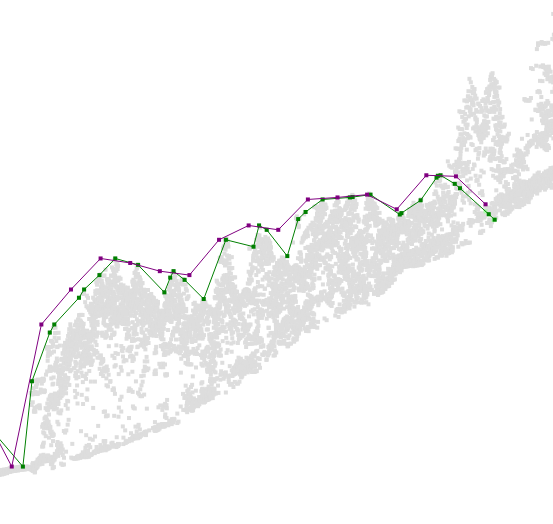
\includegraphics[width=1.0\linewidth]{tmp/hull_vs_bin.pdf} 
\caption{Comparison of surface extraction methods. Binning (purple) shows a distinct upward bias over the concave hull (green). Bin size and segment length are $\SI{10}\m$.}
\label{fig:hull_vs_bin}
\end{figure}


\section{Methods and Materials}


 In this instance, the distance to the surface is measured using a LightWare SF30/C laser rangefinder mounted on a scanning d


\newpage

\printbibliography

\end{document}